\documentclass[a4paper,12pt]{article}
\usepackage[latin1]{inputenc}
\usepackage[spanish]{babel}
\usepackage{graphicx}
\usepackage{amsmath}
\usepackage{wrapfig}
\setlength{\textheight}{250mm}
\setlength{\textwidth}{165mm}
\setlength{\topmargin}{-15mm}
\setlength{\oddsidemargin}{0pt}
\pagestyle{empty}

\begin{document}

\def\bm#1{{\mbox{\boldmath $#1$}}}
\def\eqdef{\buildrel \rm def \over =}
\def\signo{\mathop{\rm signo}\nolimits}

\mbox{}\vspace*{-20mm}

{\centering
{\small\sc Escuela T�cnica Superior de Ingenieros de Caminos, Canales y Puertos (Madrid)}\\*[4mm]
{\Large\bf M�todo de los Elementos Finitos}\\*[4mm]
PR�CTICA 5. Elementos isoparam�tricos. \\*[4mm]
}

% \vspace{4mm}

% ENUNCIADO

Un panel de canto variable, con las medidas que se indican en la figura,
est� empotrado en un extremo y sometido a esfuerzo cortante en el otro
extremo. El esfuerzo aplicado es $\bm{F}=1.8$ kN. Las propiedades el�sticas
del material del panel son $E=70$ GPa y $\nu=0.33$, y su espesor es $1$ mm.
Se considerar� la hip�tesis de tensi�n plana.

Se pide comparar los desplazamientos verticales en el extremo libre
considerando una malla de $16 \time 16$ elementos cuadril�teros de $4$
y $8$ nodos, y tri�ngulos de $3$ y $6$ nodos.

\begin{wrapfigure}{r}{50mm}
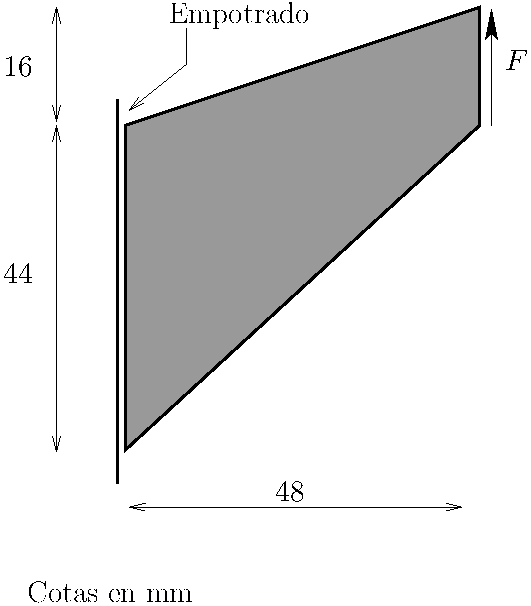
\includegraphics{cook}
\end{wrapfigure}
\end{document}
